\documentclass{handout}

% \SetInstructor{Lt Col James Phillips}
\SetCourseTitle{ECE231: Electrical Circuits and Systems I}
\SetSemester{Block II}
\SetHandoutTitle{Lecture 14: Operational Amplifiers - Part 1}
%\SetDueDate{1 Jan 2016}
%\ShowAllBlanks

\showsoln \setsolncolor{red}

\begin{document}
\maketitle

\textbf{OBJECTIVES:}
\begin{enumerate}
\item Understand Op Amp Basics
\item Understand the ideal Op Amp model
\item Apply the Ideal Op Amp model to derive inverting and non-inverting op amp circuits
\end{enumerate}

\textbf{READING}
\begin{description}
\item [Required]:
\begin{itemize}
\item  Textbook, sections 4.3--4.4, pages 177--190
\end{itemize}
\item [Optional]: None
\end{description}

\section{Operational Amplifier (or Op Amp) basics}
\subsection{The very basics}
\soln{2in}{
\begin{enumerate}
\item An Op Amp is an active device
\item Because it is an active device it has an external power supply
\item Op Amps are 5-terminal devices: 2 inputs, 2 power supplies and 1 output
\item OpAmps have very high gain
\end{enumerate}
}

\newpage
\clearpage
\pagebreak

\subsection{Op Amp Schematic \& Notation}
\begin{figure} [h! t! b!]
\centering
\soln{2.5in}{
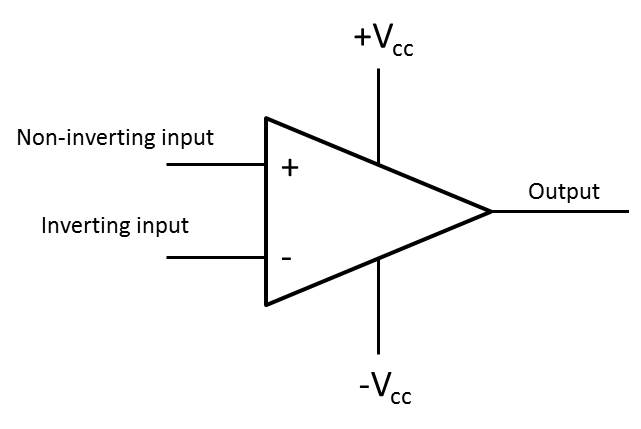
\includegraphics[width=0.5\textwidth]{FullOpAmp.jpg}
}
\caption{Op Amp showing all five terminals}
\label{fig: FullOpAmp}
\end{figure}

Figure \ref{fig: FullOpAmp} shows the schematic for an Op Amp with all five terminals labeled.  Notice there is both a positive and negative power supply (labeled $+V_{cc}$ and $-V_{cc}$ respectively).  Also notice the inputs are labeled as inverting and non-inverting; the reason for this will be obvious soon.

Most of the time in schematics, we suppress the power supplies and illustrate the Op Amp as shown in Figure \ref{fig: OpAmp}.
\begin{figure} [h! t! b!]
\centering
\soln{2in}{
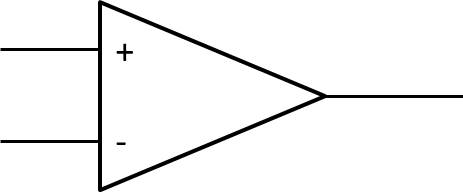
\includegraphics[width=0.5\textwidth]{OpAmp.jpg}
}
\caption{Op Amp showing only input and output terminals}
\label{fig: OpAmp}
\end{figure}

\subsection{Op Amp Transfer Characteristics}
By transfer charateristics, we are refering to the relationship between the {\em inverting}, the {\em non-inverting}, and the {\em output} terminals.  In Figure \ref{fig: OpAmp2}, the voltage (relative to common ground) of each terminal is labeled; the gain $A$  is also shown, typically $A>10^5$.  The relationship between the voltages at the terminals is:
\begin{equation}
v_O=A(v_p-v_n)
\end{equation}

\begin{figure} [h! t! b!]
\centering
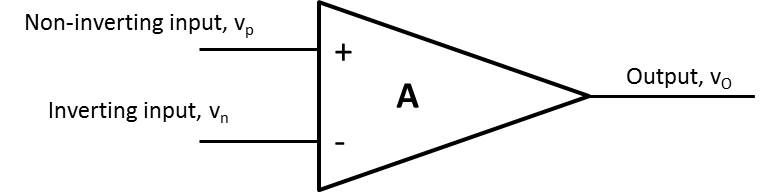
\includegraphics[width=0.5\textwidth]{OpAmp2.jpg}
\caption{Op Amp with terminal voltages  and gain labeled}
\label{fig: OpAmp2}
\end{figure}

Op Amps have two operations regions:
\begin{description}
\item[Linear mode] -- The Op Amp is operating lineraly whenever $A|v_p-v_n|<V_{cc}$; the output relationship is $v_O=A(v_p-v_n)$
\item[Saturation mode] -- The Op Amp is saturated when $A|v_p-v_n|>+V_{cc}$; the output will be $v_O=+V_{cc}$ if $A(v_p-v_n)>+V_{cc}$.  If $A(v_p-v_n)<-V_{cc}$ then the output is $v_O=-V_{cc}$.
\end{description}

\subsection{The ideal Op Amp}
Four our purposes we are going to always assume {\em Ideal Operational Amplifiers} in our calculation; so we need to give some operationg characteristics of an ideal Op Amp.

\begin{figure} [h! t! b!]
\centering
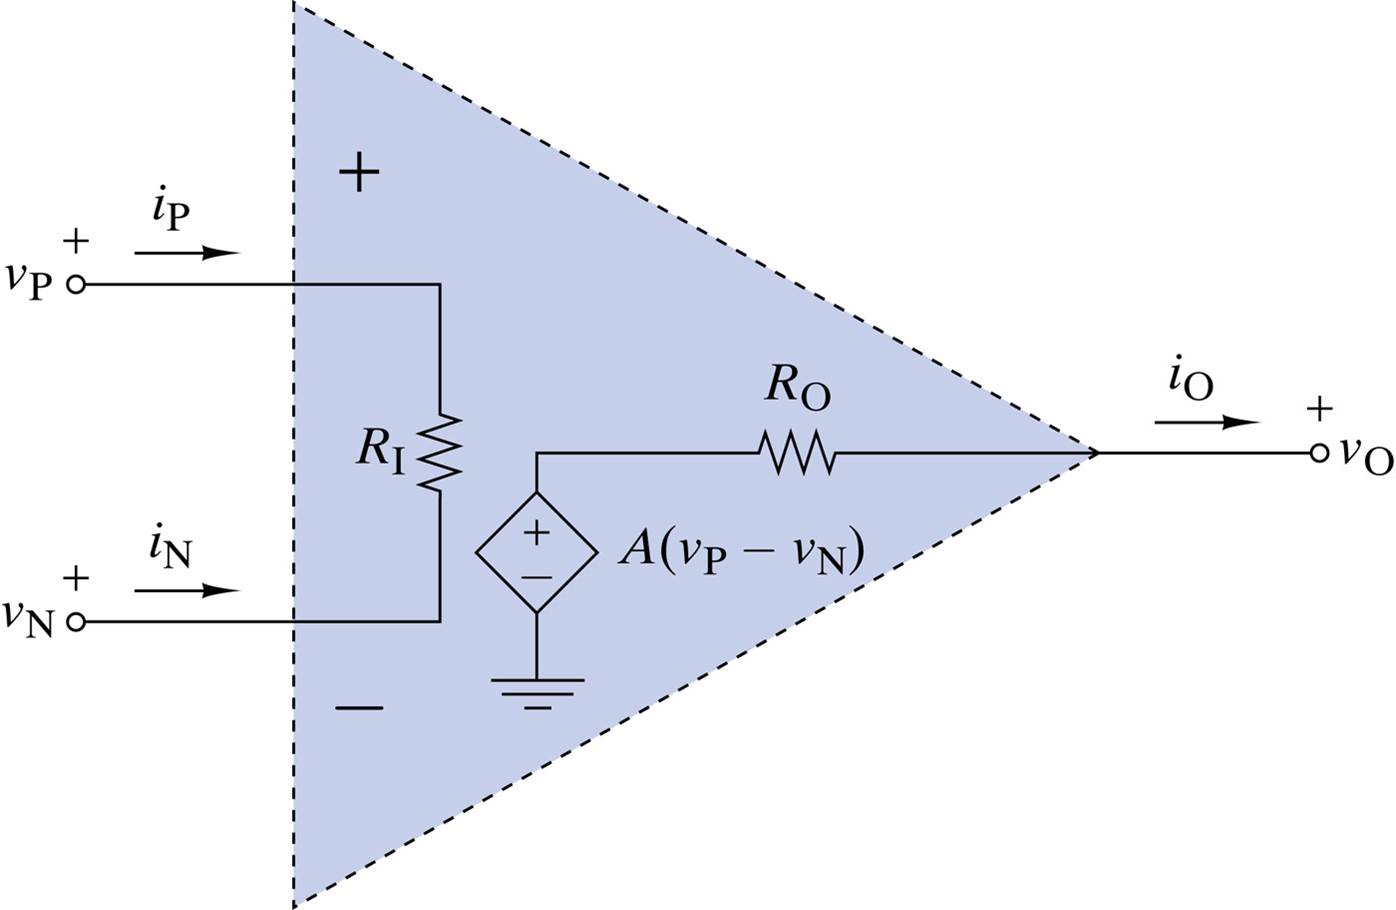
\includegraphics[width=0.5\textwidth]{IdealOpAmpModel.jpg}
\caption{Ideal Op Amp model}
\label{fig: IdealOpAmp}
\end{figure}

Characteristics of ideal Op Amps (reference Figure \ref{fig: IdealOpAmp}):
\soln{2in}{
\begin{enumerate}
\item Ideal Op Amps have infinite gain
\item Zero current flows into the input terminals, $i_p=i_n=0$
\item There is no voltage difference between the input terminals, $v_p=v_n$
\item Input resistance is infinite, $R_I=\infty$
\item Output resistance is zero, $R_O=0$
\end{enumerate}
}

We will take advantage of these assumptions in the next few sections to develop some common Op Amp circuits; specifically the inverting  and non-inverting amplifiers.  Next lesson we will develop circutis for Summing and Subtracting amplifiers.

\newpage
\clearpage
\pagebreak

\section{Non-Inverting Op Amps}
Figure \ref{fig: NonInvertingOpAmp} shows a schematic for a non-inverting amplifier circuit.  In each of the circuits we analyze moving forward it is important to note a couple of things:
\soln{2in}{
\begin{enumerate}
\item The gain, $K$, of the circuit, is not the same as the gain of the amplifier, $A$
\item We will use the term Amplifier or Op Amp to sometimes refer to the device and sometimes to the circuit; pay attention to context
\end{enumerate}
}

\begin{figure}
\centering
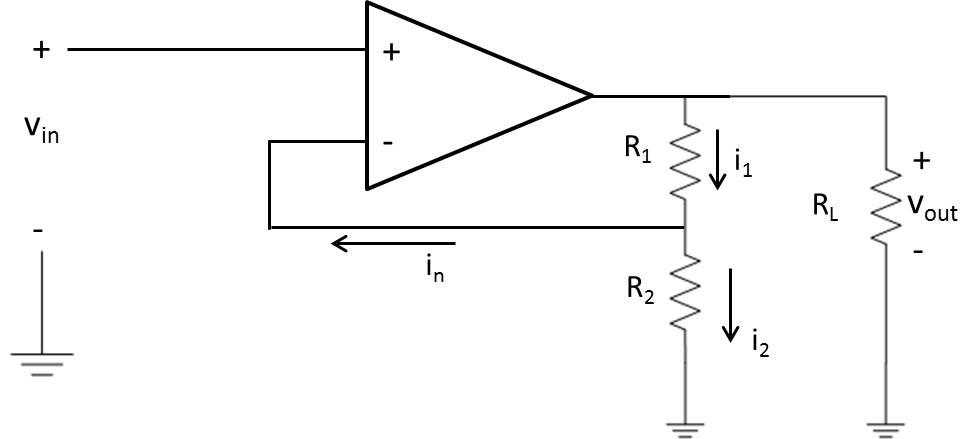
\includegraphics[width=0.5\textwidth]{NonInvertingOpAmp.jpg}
\caption{Non-Inverting Op Amp}
\label{fig: NonInvertingOpAmp}
\end{figure}

\subsection{Derivation of Non-inverting Op Amp Transfer characteristic}
The derviation will continue to refer to Figure \ref{fig: NonInvertingOpAmp}.

To start the derivation (and almost any Op Amp derivation), we write the KCL equation at the inverting terminal:
\soln{2in}{
\begin{equation}
i_1=i_2+i_n
\end{equation}
but we know, for ideal op amps, $i_n=0$, so
\begin{equation}
i_1=i_2
\end{equation}

Also take note that current into the non-inverting terminal is also zero; this will become important later when we talk about stage loading.
}

Next, write an expression for the voltage across $R_2$
\soln{2in}{
\begin{equation}
V_{R2}=i_2R_2
\end{equation}
but we know that the voltage between the op amp input terminals is zero, so $V_{R2}=V_{in}$ therefore
\begin{equation}
V_{in}=i_2R_2
\end{equation}
}

We can now solve for the currents, $i_1$ and $i_2$
\soln{2in}{
\begin{equation}
i_2=\frac{V_{in}}{R_2}
\end{equation}
and since $i_1=i_2$
\begin{equation}
i_1=\frac{V_{in}}{R_2}
\end{equation}
}
We can know write an expression for $V_{out}$ by recognizing that
\soln{2in}{
\begin{equation}
V_{out} = V_{R1} + V_{R2}
\end{equation}
which equals (I will leave the algebra to you)
\begin{equation}
V_{out} = V_{in}\frac{R1+R2}{R2}
\end{equation}
}
This yields a gain of the non-inverting amplifier of
\begin{equation}
K=\frac{R_1+R_2}{R_2}
\end{equation}

\subsection{Examples}
\textbf{Example 1 - Textbook Exercise 4-15} -- If a non-inverting amplifier circuit is operating with $R_1=2R_2$ and a $V_{cc}=\pm 12$ , what is the gain?  For what input voltages is it operating in the linear mode?

\soln{3.5in}{
Our gain equation for a non-inverting amplifier is
\begin{equation}
K=\frac{R_1+R_2}{R_2}
\end{equation}
If $R_1=2R_2$ then the gain becomes
\begin{equation}
K=\frac{2R_2+R_2}{R_2}=3
\end{equation}
For the amplifier to operate in linear mode.
\begin{equation}
|KV_{in}|<|V_{cc}|
\end{equation}
therefore
\begin{equation}
|V_{in}|<4\ V
\end{equation}

}

\textbf{Example 2} -- Design an inverting amplifier with a gain of $K=30\ \ \pm10\%$ using standard resistance values.
\soln{3.5in}{
To design the amplifier we really just have to chose values for $R_1$ and $R_2$ to satisfy
\begin{equation}
30 \pm 10\%= \frac{R_1+R_2}{R_2}
\end{equation}
to that end, let's select $R_2=1.5\ k\Omega$ and solve the following exact equation
\begin{equation}
30 = \frac{R_1 + 1.5\ k\Omega}{1.5\ k\Omega}
\end{equation}
which yields
\begin{equation}
R_1=43.5\ k\Omega
\end{equation}
The closest standard resistance value is $43\ k\Omega$ which gives a gain of
\begin{equation}
K=\frac{43\ k\Omega+1.5\ k\Omega}{1.5\ k\Omega} = 29.667
\end{equation}
This is easily within 10 \% of $K=30$

}

\newpage
\clearpage
\pagebreak

\section{Inverting Op Amps}
Figure \ref{fig: InvertingOpAmp} shows a schematic for a inverting amplifier circuit.

\begin{figure}
\centering
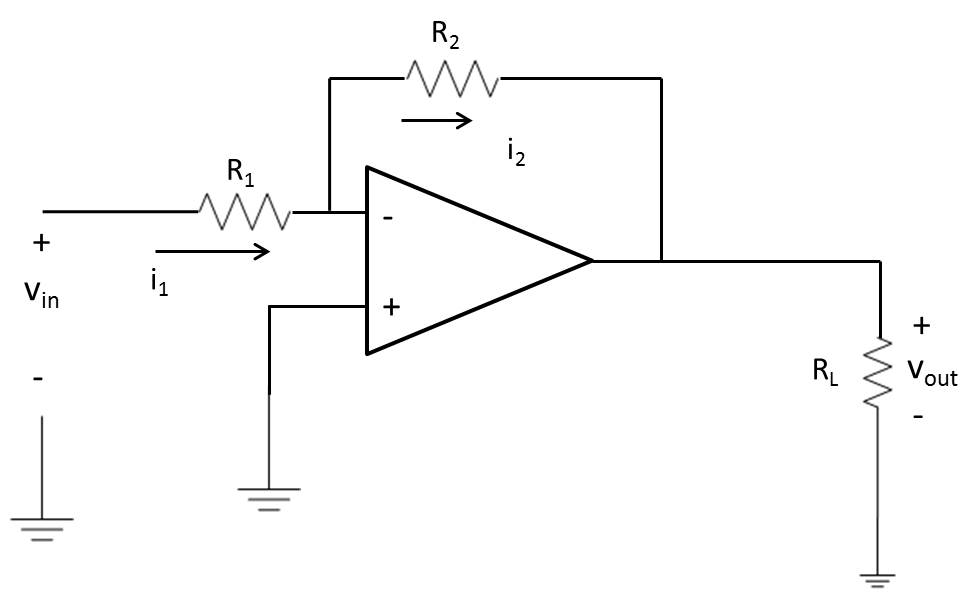
\includegraphics[width=0.6\textwidth]{InvertingOpAmp.jpg}
\caption{Inverting Op Amp}
\label{fig: InvertingOpAmp}
\end{figure}

\subsection{Derivation of Inverting Op Amp Transfer characteristic}
The derviation will continue to refer to Figure \ref{fig: InvertingOpAmp}.

Key parameters not labeled on the diagram (these always apply so I will habitually not label them):
\begin{itemize}
\item $i_n$ \& $i_p$ are the currents \textbf{into} the inverting terminal and non-inverting terminals
\item $v_n$ \& $v_p$ are the voltages between the inverting and non-inverting terminals and ground
\end{itemize}

\textbf{Step 1:}  Write KCL equation for the inverting terminal
\soln{2in}{
\begin{equation}
i_1=i_2+i_n
\end{equation}
but we know $i_n=0$ from the ideal Op Amp definition, therefore:
\begin{equation}
i_1=i_2
\end{equation}
}

\textbf{Step 2:} Next, we can write expressions for $i_1$ and $i_2$ in terms of input and output voltages ($V_{in}$ \& $V_{out}$)
\soln{2in}{
\begin{equation}
i_1 = \frac{V_{in} - v_n}{R_1}
\end{equation}

\begin{equation}
i_2 = \frac{v_n - V_{out}}{R_2}
\end{equation}
but we know $v_n=0$ from the ideal Op Amp definition, therefore:
\begin{equation}
i_1 = \frac{V_{in}}{R_1}
\end{equation}
\begin{equation}
i_2 = \frac{-V_{out}}{R_2}
\end{equation}
}

\textbf{Step 3:} Since step 1 told us that $i_1=i_2$, set the expressions from step to equal to one another and solve for $K=\frac{V_{out}}{V_{in}}$

\soln{2in}{
\begin{equation}
\frac{V_{in}}{R_1}=\frac{-V_{out}}{R_2}
\end{equation}
solving for $\frac{V_{out}}{V_{in}}$ gives
\begin{equation}
\frac{V_{out}}{V_{in}}=\frac{-R_2}{R_1}
\end{equation}
}

\subsection{Examples}
\textbf{Textbook Design Exercise 4-20}
A $2\ mV$ signal needs to be amplified by a gain of $K=-450 \pm 10\%$.  Design an appropriate Op Amp circuit using standard resistor values

\soln{3.5in}{
Since the required gain is negative is should be clear we need an {\em inverting} amplifier.  Recall, the gain for an inverting amplifier is
\begin{equation}
K=\frac{-R_2}{R_1}
\end{equation}
We can play around with different values of $R_1$ and $R_2$ to find a value of $K$ that is close to $-450$.  The closest I was able to come up with was $R_1 = 1.8\ k\Omega$ and $R_2 = 820\ k\Omega$ which gives a gain of
\begin{equation}
K=\frac{-820\ k\Omega}{1.8\ k\Omega} = -455.556
\end{equation}
easily inside the $10\%$ tolerance.

Notice the chosen resistors are in the range of $1\ k\Omega$ to $1\ M\Omega$.  Bigger or smaller than that can have some adverse effects that we will discuss later.
}

\textbf{Example 3 - Textbook Exercise 4-19}--Find $V_{out}$ of an inverting amplifier with $R_1= 10\ k\Omega$  and $R_2= 33\ k\Omega$ when $V_{in}= 2\ V$. What about when $V_{in} = 4\ V$ and $V_{in} = 6\ V$.  $V_{cc} = \pm15\ V$

\soln{3.5in}{
First calculate the gain
\begin{equation}
K=\frac{-33\ k\Omega}{10\ k\Omega} = -3.3
\end{equation}

For $V_{in}= 2\ V$,
\begin{equation}
V_{out} = -3.3 \times 2\ V=-6.6\ V
\end{equation}

For $V_{in}= 4\ V$,
\begin{equation}
V_{out} = -3.3 \times 4\ V=-13.2\ V
\end{equation}

For $V_{in}= 6\ V$,
\begin{equation}
V_{out} = -3.3 \times 6\ V=-19.8\ V
\end{equation}
but this saturates the amplifier and we only get $-15\ V$ output.
}

\newpage
\clearpage
\pagebreak

\subsection{Input loading of in Inverting Amplifier}
Since an inverting amplifier has an external resistor (with a current flowing) on the input, we will have to look at the effects of {\em loading}.  Any resistance attached to the input will ``add'' to the input resistance ($R_1$)and change the gain of the amplifier circuit.  Before we move to an example, notice that this is not a problem with non-inverting amplifiers since there is not an external resistor attached to the input.

\textbf{Example 4} A non-ideal $12\ V$ source that has an internal resistance of $50 \Omega$ is attached to a Inverting Op Amp with $R_1 = 1\ k\Omega$ and $R_2 = 10\ k\Omega$.  What is the ideal gain, $K$, of the amplifier? What are the actual values of $K$ and $V_{out}$? If $R_1 = 100\ \Omega$ and $R_2 = 1\ k\Omega$ What is the ideal gain?  What are the actual values of $K$ and $V_{out}$?

\soln{6in}{
The ideal gain of the amplifier is for the $R_1 = 1\ k\Omega$ and $R_2 = 10\ k\Omega$ is
\begin{equation}
K=\frac{-10\ k\Omega}{1\ k\Omega} = -10
\end{equation}

To calculate the actual value of the gain, you must recognize that the internal resistance of the source adds in series to the input resistor giving
\begin{equation}
K=\frac{-10\ k\Omega}{1\ k\Omega + 50 \Omega} = -9.524
\end{equation}
which yields a $V_{out} = 114.4\ V$

The ideal gain of the amplifier is for the $R_1 = 100\ \Omega$ and $R_2 = 1\ k\Omega$ is
\begin{equation}
K=\frac{-1\ k\Omega}{100\ \Omega} = -10
\end{equation}

To calculate the actual value of the gain, you must recognize that the internal resistance of the source adds in series to the input resistor giving
\begin{equation}
K=\frac{-1\ k\Omega}{100\ \Omega + 50 \Omega} = -6.667
\end{equation}
which yields a $V_{out} = 80\ V$

Notice the effects of {\em loading} on an inverting amplifier.

}


\newpage
\clearpage
\pagebreak

\newpage
\clearpage
\pagebreak

\newpage
\clearpage
\pagebreak

\newpage
\clearpage
\pagebreak

\newpage
\clearpage
\pagebreak

\end{document}


% Equation Array Example Code
%\begin
%{eqnarray}
%P_R &=& i_R^2R \nonumber \\
%P_R &=& (100\ mA)^2 \times 100\ \Omega \nonumber \\
%P_R &=& (100 \times 10^{-3}\ A)^2 \times 100\ \Omega \\
%P_R &=& 10000 \times 10^{-6}\ A^2  \times 100\ \Omega \nonumber \\
%P_R &=& 1\ W  \nonumber
%\end{eqnarray}

% Figure Example Code
%\begin{figure} [h! t! b!]
%\centering
%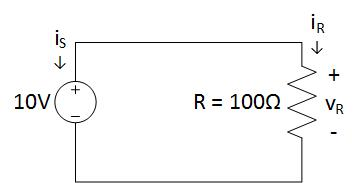
\includegraphics[width=0.5\textwidth]{OhmsLawExampleSolution.jpg}
%\caption{Ohm's Law example circuit}
%\label{fig: OhmsLawExampleSolution}
%\end{figure}

%Table Example Code
%\begin{table}[h]
%\centering
%\begin{tabular}{|l|c|c|}
%\hline
%Prefix & Abbreviation & Value \\
%\hline \hline
%Giga & $G$ & $10^9$ \\
%Mega & $M$ & $10^6$ \\
%Kilo & $k$ & $10^3$ \\
%\hline
%milli & $m$ & $10^{-3}$ \\
%micro & $\mu$ & $10^{-6}$ \\
%nano & $n$ & $10^{-9}$ \\
%pico & $p$ & $10^{-12}$ \\
%\hline
%\end{tabular}
%\caption{Engineering prefixes and values}
%\label{tab: Eng Prefixes}
%\end{table}
